\chapter{Opportunities For Interventions: Making the Field More Equitable}


\section{Introduction}


\begin{figure}[ht]
\centering
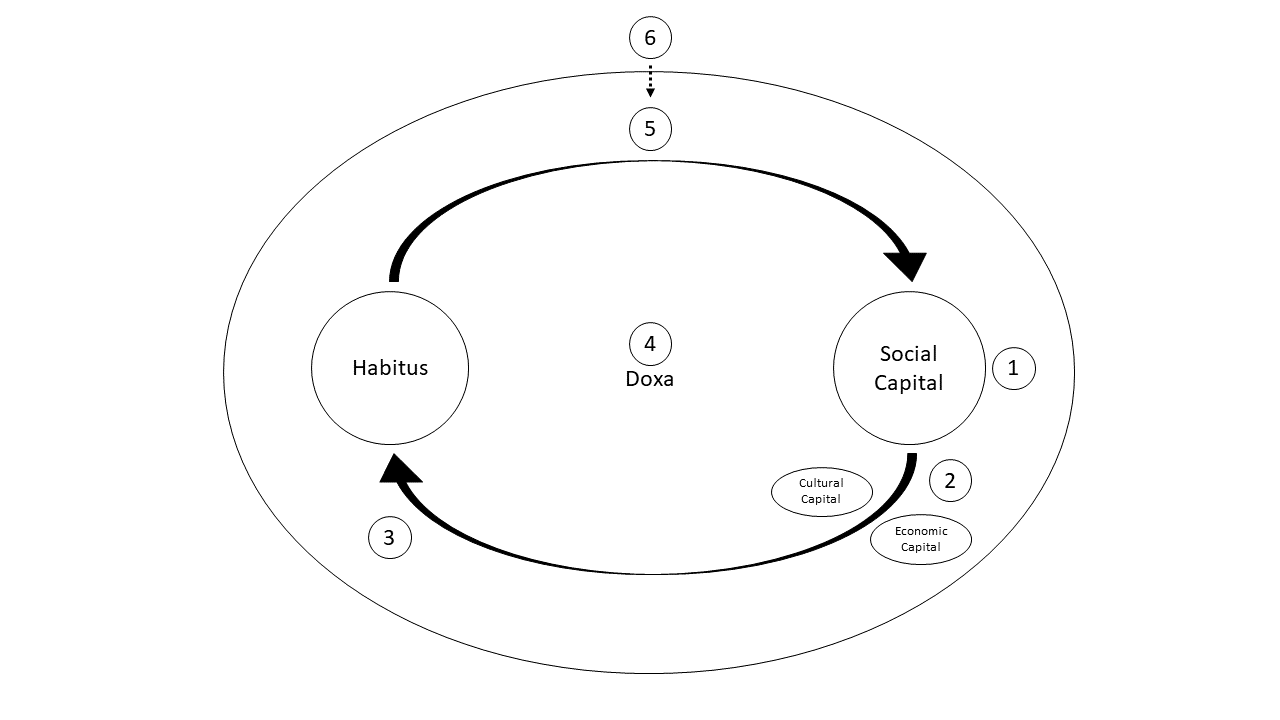
\includegraphics[width=\textwidth]{HabitusSocCap_TheoreticalModel.png}
\caption{\label{fig:HabitusSocCap_TheoreticalModel_C7}\textbf{Complete Theoretical Model}. The complete theoretical model. The model, informed by the described experiences of university science students, expands on the interaction between habitus and capital originally illustrated by \cite{Bourdieu1984}. The model provides a step by step description of how social capital translates into habitus transformation, and how habitus generates future capital accumulation. Step 1 refers to the initial availability of social capital for an individual. Step 2 refers to the value gained through leveraging social capital into forms of economic and cultural capital. Step 3 refers to how social capital is internalised by the individual. Step 4 refers to how habitus informs the acquisition of future social capital. 5 refers to factors outside of the individual that structure the field (by availability of capital and exchange value).}
\end{figure}

\section{1: Social Capital in the Field of University Science}
This section discusses the availability of social relationships that participants had in the field of university science. These relationships are categorised into three key groups, social capital through family connections, social capital through lecturers, and social capital through peers. 

\subsection{Direction: Increase Availability of Connections}
It may be possible to address equity issues by increasing the availability of these relationships to students who would not have access to them in their everyday life. Interventions, provided by institutional support services or groups outside of institutions, can mobilise structural changes in the field by increasing the availability of connections. 


\section{2: Leveraging Social Capital}
The value of social capital is derived from the economic and cultural capital that can be mobilised through connections with others. These resources may provide students with advantages in supporting their learning and providing student access to information about the field. 


\subsection{Direction: Place Value on Alternative Forms of Cultural Capital}


\section{3: Internalising Capital}
The capital that students accrue in university science not only provides access to resources, but it can also influences the way that students see themselves in the field. Capital, which determines students position in the field, is internalised by students via their habitus, which establishes the students disposition towards the field \cite{Bourdieu1992}. Students who hold high levels of social capital may feel an affinity with the field and see progression to university as a path already drawn out.


\subsection{Direction: Provide Counterspaces}


\section{4: Doxa (Societal Discourses)}
Outside of the of the social relationships that students hold, general discourses in society influence the development of habitus.

\subsection{Direction: Combat Negative Doxa}

\section{5: Generating Social Capital}
The future acquisition of social capital is informed by habitus.

\subsection{Direction: Reduce the Perceived Power Imbalance}


\section{6: Institutional Habitus}
The cycle is impacted on by interventions operating in the field, which themselves are directed by an institutional habitus.


\subsection{Direction: Equity Charters and Movements}


\section{Conclusion}


